% Options for packages loaded elsewhere
\PassOptionsToPackage{unicode}{hyperref}
\PassOptionsToPackage{hyphens}{url}
\PassOptionsToPackage{dvipsnames,svgnames,x11names}{xcolor}
%
\documentclass[
  letterpaper,
  DIV=11,
  numbers=noendperiod]{scrartcl}

\usepackage{amsmath,amssymb}
\usepackage{iftex}
\ifPDFTeX
  \usepackage[T1]{fontenc}
  \usepackage[utf8]{inputenc}
  \usepackage{textcomp} % provide euro and other symbols
\else % if luatex or xetex
  \usepackage{unicode-math}
  \defaultfontfeatures{Scale=MatchLowercase}
  \defaultfontfeatures[\rmfamily]{Ligatures=TeX,Scale=1}
\fi
\usepackage{lmodern}
\ifPDFTeX\else  
    % xetex/luatex font selection
\fi
% Use upquote if available, for straight quotes in verbatim environments
\IfFileExists{upquote.sty}{\usepackage{upquote}}{}
\IfFileExists{microtype.sty}{% use microtype if available
  \usepackage[]{microtype}
  \UseMicrotypeSet[protrusion]{basicmath} % disable protrusion for tt fonts
}{}
\makeatletter
\@ifundefined{KOMAClassName}{% if non-KOMA class
  \IfFileExists{parskip.sty}{%
    \usepackage{parskip}
  }{% else
    \setlength{\parindent}{0pt}
    \setlength{\parskip}{6pt plus 2pt minus 1pt}}
}{% if KOMA class
  \KOMAoptions{parskip=half}}
\makeatother
\usepackage{xcolor}
\setlength{\emergencystretch}{3em} % prevent overfull lines
\setcounter{secnumdepth}{-\maxdimen} % remove section numbering
% Make \paragraph and \subparagraph free-standing
\ifx\paragraph\undefined\else
  \let\oldparagraph\paragraph
  \renewcommand{\paragraph}[1]{\oldparagraph{#1}\mbox{}}
\fi
\ifx\subparagraph\undefined\else
  \let\oldsubparagraph\subparagraph
  \renewcommand{\subparagraph}[1]{\oldsubparagraph{#1}\mbox{}}
\fi


\providecommand{\tightlist}{%
  \setlength{\itemsep}{0pt}\setlength{\parskip}{0pt}}\usepackage{longtable,booktabs,array}
\usepackage{calc} % for calculating minipage widths
% Correct order of tables after \paragraph or \subparagraph
\usepackage{etoolbox}
\makeatletter
\patchcmd\longtable{\par}{\if@noskipsec\mbox{}\fi\par}{}{}
\makeatother
% Allow footnotes in longtable head/foot
\IfFileExists{footnotehyper.sty}{\usepackage{footnotehyper}}{\usepackage{footnote}}
\makesavenoteenv{longtable}
\usepackage{graphicx}
\makeatletter
\def\maxwidth{\ifdim\Gin@nat@width>\linewidth\linewidth\else\Gin@nat@width\fi}
\def\maxheight{\ifdim\Gin@nat@height>\textheight\textheight\else\Gin@nat@height\fi}
\makeatother
% Scale images if necessary, so that they will not overflow the page
% margins by default, and it is still possible to overwrite the defaults
% using explicit options in \includegraphics[width, height, ...]{}
\setkeys{Gin}{width=\maxwidth,height=\maxheight,keepaspectratio}
% Set default figure placement to htbp
\makeatletter
\def\fps@figure{htbp}
\makeatother

\KOMAoption{captions}{tableheading}
\makeatletter
\makeatother
\makeatletter
\makeatother
\makeatletter
\@ifpackageloaded{caption}{}{\usepackage{caption}}
\AtBeginDocument{%
\ifdefined\contentsname
  \renewcommand*\contentsname{Table of contents}
\else
  \newcommand\contentsname{Table of contents}
\fi
\ifdefined\listfigurename
  \renewcommand*\listfigurename{List of Figures}
\else
  \newcommand\listfigurename{List of Figures}
\fi
\ifdefined\listtablename
  \renewcommand*\listtablename{List of Tables}
\else
  \newcommand\listtablename{List of Tables}
\fi
\ifdefined\figurename
  \renewcommand*\figurename{Figure}
\else
  \newcommand\figurename{Figure}
\fi
\ifdefined\tablename
  \renewcommand*\tablename{Table}
\else
  \newcommand\tablename{Table}
\fi
}
\@ifpackageloaded{float}{}{\usepackage{float}}
\floatstyle{ruled}
\@ifundefined{c@chapter}{\newfloat{codelisting}{h}{lop}}{\newfloat{codelisting}{h}{lop}[chapter]}
\floatname{codelisting}{Listing}
\newcommand*\listoflistings{\listof{codelisting}{List of Listings}}
\makeatother
\makeatletter
\@ifpackageloaded{caption}{}{\usepackage{caption}}
\@ifpackageloaded{subcaption}{}{\usepackage{subcaption}}
\makeatother
\makeatletter
\@ifpackageloaded{tcolorbox}{}{\usepackage[skins,breakable]{tcolorbox}}
\makeatother
\makeatletter
\@ifundefined{shadecolor}{\definecolor{shadecolor}{rgb}{.97, .97, .97}}
\makeatother
\makeatletter
\makeatother
\makeatletter
\makeatother
\ifLuaTeX
  \usepackage{selnolig}  % disable illegal ligatures
\fi
\IfFileExists{bookmark.sty}{\usepackage{bookmark}}{\usepackage{hyperref}}
\IfFileExists{xurl.sty}{\usepackage{xurl}}{} % add URL line breaks if available
\urlstyle{same} % disable monospaced font for URLs
\hypersetup{
  pdftitle={Designing Population Health Studies},
  colorlinks=true,
  linkcolor={blue},
  filecolor={Maroon},
  citecolor={Blue},
  urlcolor={Blue},
  pdfcreator={LaTeX via pandoc}}

\title{Designing Population Health Studies}
\usepackage{etoolbox}
\makeatletter
\providecommand{\subtitle}[1]{% add subtitle to \maketitle
  \apptocmd{\@title}{\par {\large #1 \par}}{}{}
}
\makeatother
\subtitle{April 6 and April 8 Eric Delmelle}
\author{}
\date{}

\begin{document}
\maketitle
\ifdefined\Shaded\renewenvironment{Shaded}{\begin{tcolorbox}[interior hidden, frame hidden, enhanced, borderline west={3pt}{0pt}{shadecolor}, sharp corners, boxrule=0pt, breakable]}{\end{tcolorbox}}\fi

\begin{figure}

{\centering \includegraphics[width=3.40625in,height=\textheight]{imgs/chapter6.png}

}

\end{figure}

\hypertarget{chapter-overview}{%
\section{\texorpdfstring{{Chapter
Overview}}{Chapter Overview}}\label{chapter-overview}}

\begin{itemize}
\tightlist
\item
  Research design fundamentals in epidemiology and public health\\
\item
  Measurement validity and reliability\\
\item
  Error and bias in population health research\\
\item
  Study design approaches:

  \begin{itemize}
  \tightlist
  \item
    Cross-sectional\\
  \item
    Case-control\\
  \item
    Cohort\\
  \item
    Experimental\\
  \end{itemize}
\item
  Qualitative methods and their integration with quantitative
  approaches\\
\item
  Ethical considerations in population health research
\end{itemize}

\begin{center}\rule{0.5\linewidth}{0.5pt}\end{center}

\hypertarget{a-matter-of-measurement}{%
\subsection{\texorpdfstring{{1} {A Matter of
Measurement}}{1 A Matter of Measurement}}\label{a-matter-of-measurement}}

\hypertarget{primary-vs.-secondary-data}{%
\subsubsection{Primary vs.~Secondary
Data}\label{primary-vs.-secondary-data}}

\textbf{{Primary data}:}\\
- Data collected specifically for the purpose of the study.

\textbf{{Secondary data}:}\\
- Data collected for other purposes but reorganized and reanalyzed.

\textbf{Examples:}\\
- Health insurance claims data\\
- Employment records\\
- National health surveys

\begin{center}\rule{0.5\linewidth}{0.5pt}\end{center}

\hypertarget{primary-vs.-secondary-data-1}{%
\subsection{\texorpdfstring{{2} {Primary vs.~Secondary
Data}}{2 Primary vs.~Secondary Data}}\label{primary-vs.-secondary-data-1}}

\begin{itemize}
\tightlist
\item
  \textbf{Primary data}

  \begin{itemize}
  \tightlist
  \item
    Collected specifically for a new study
  \item
    Controlled by the researcher
  \item
    Tailored to answer specific research questions
  \end{itemize}
\item
  \textbf{Secondary data}

  \begin{itemize}
  \tightlist
  \item
    Pre-existing data collected for another purpose
  \item
    Often large-scale and readily available
  \item
    May require cleaning or transformation
  \end{itemize}
\end{itemize}

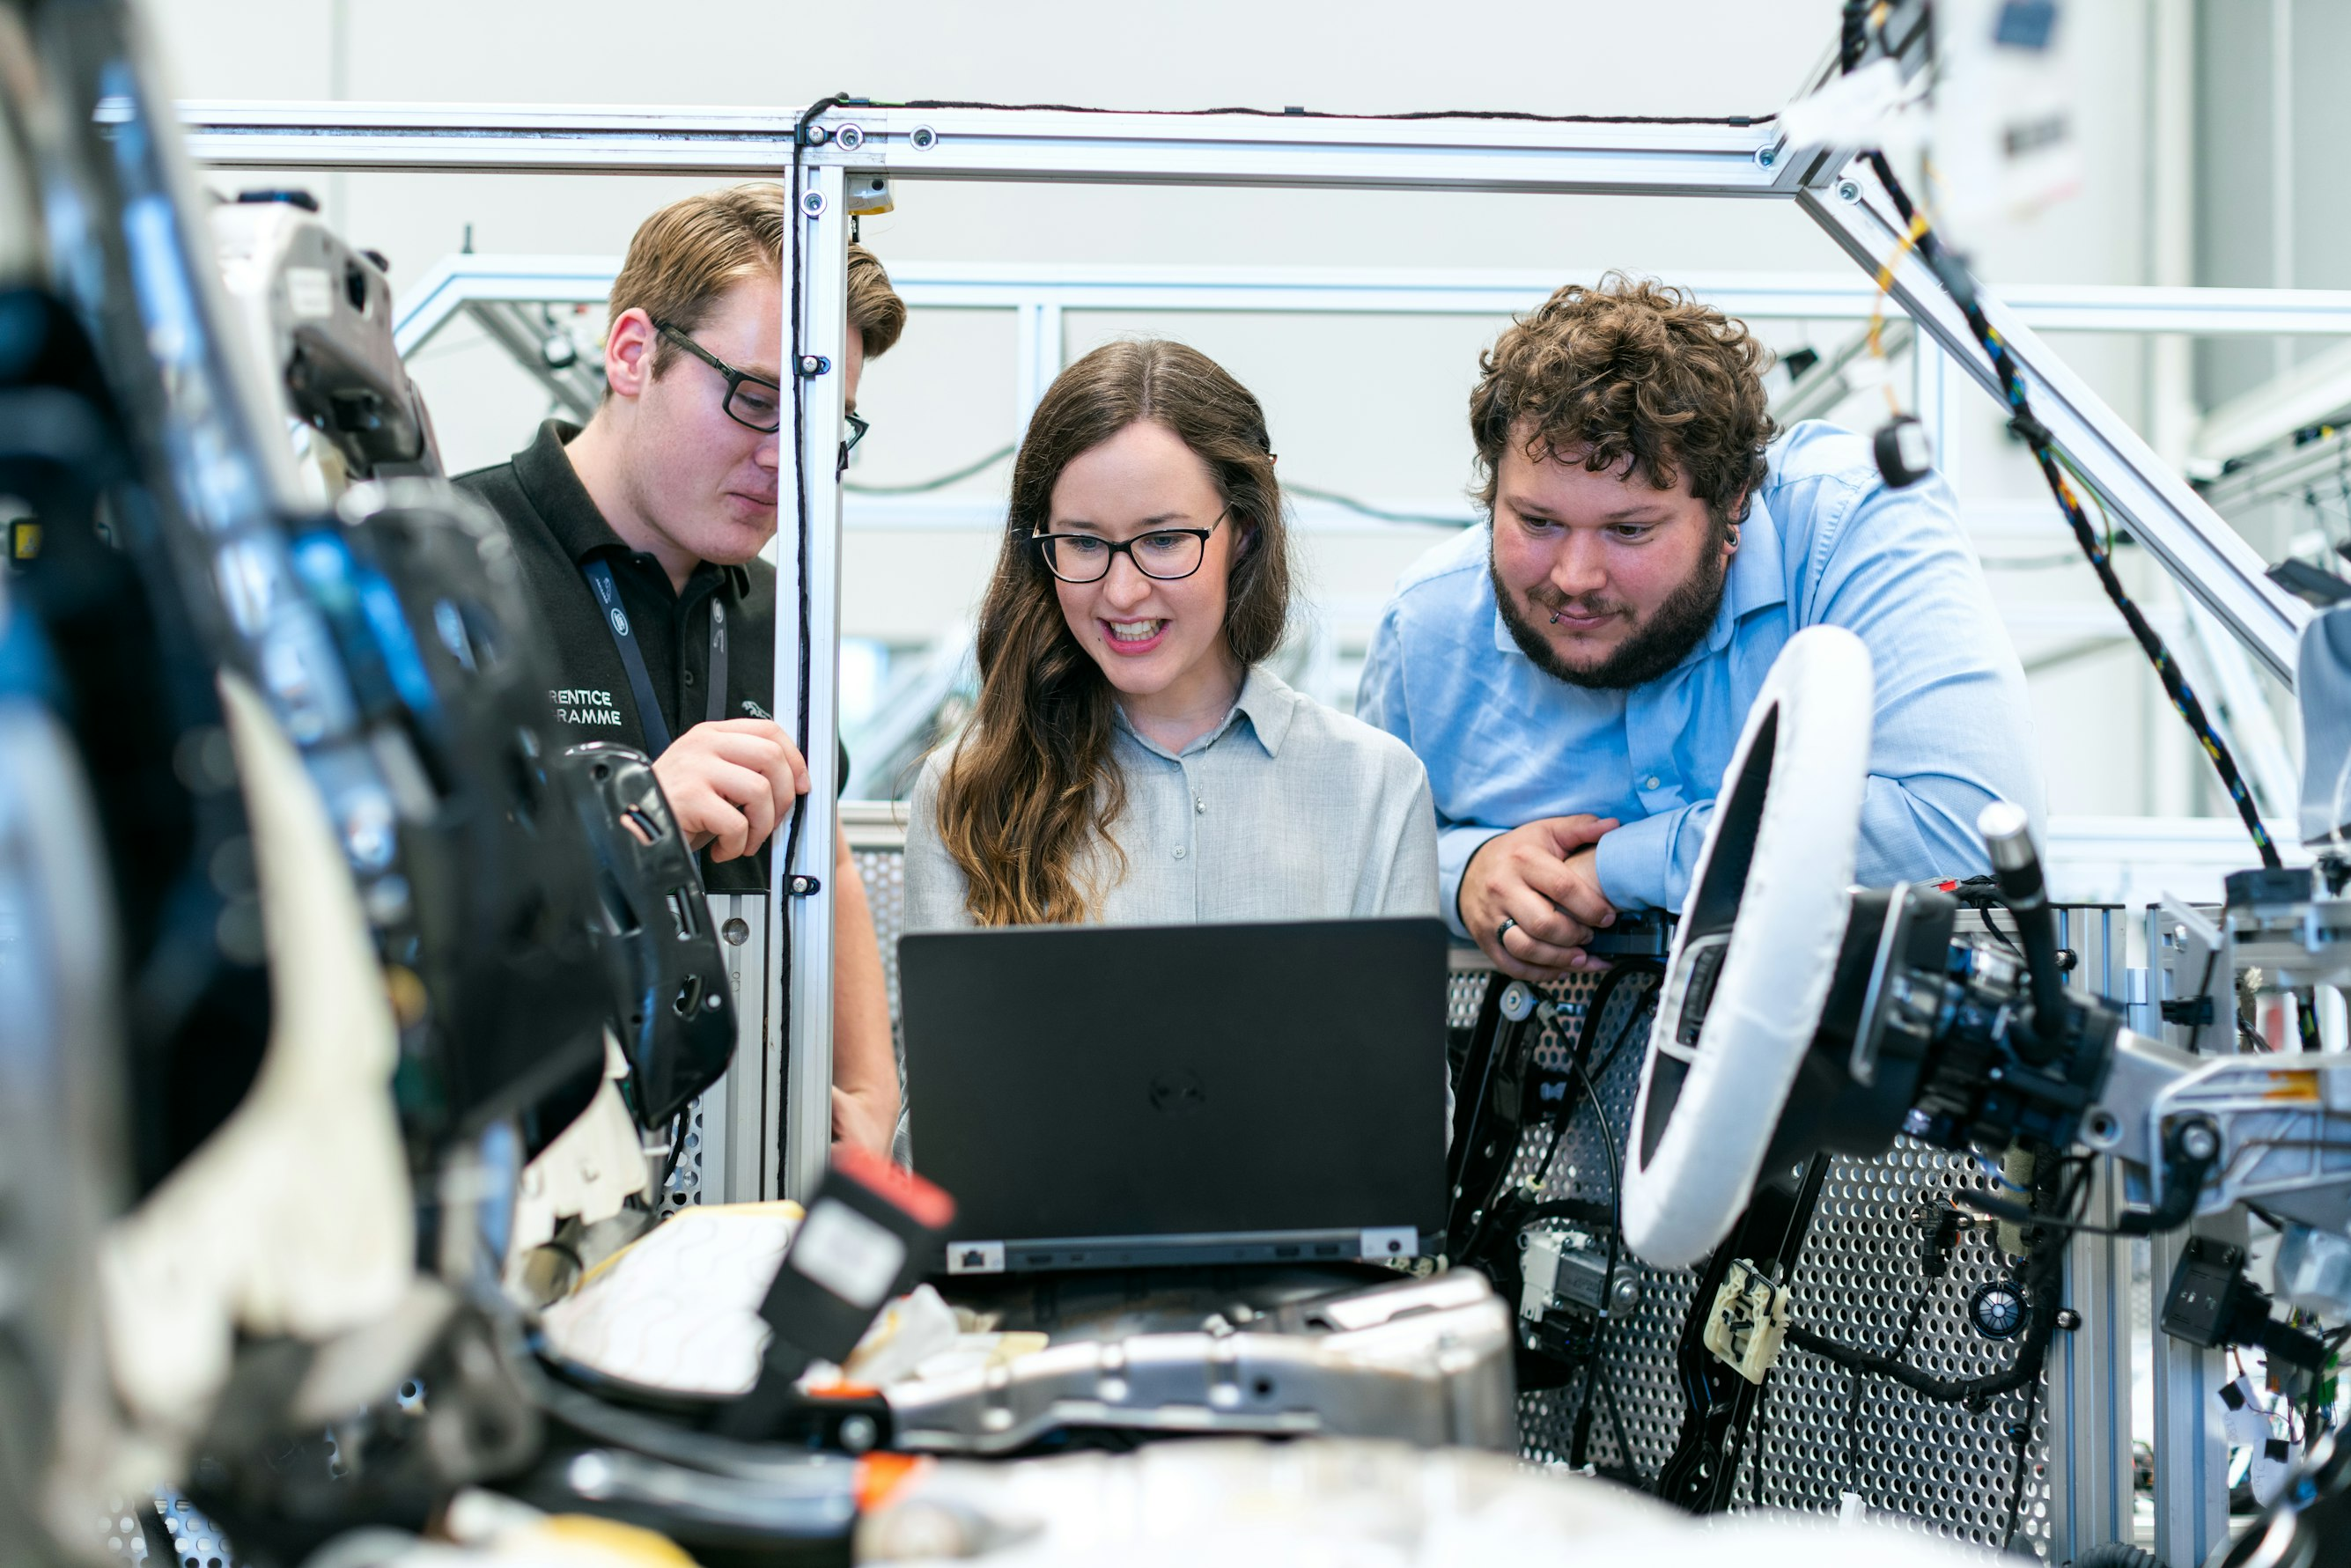
\includegraphics{index_files/mediabag/photo-1581091226033-.jpg}

While primary data offers control and precision, secondary data can save
time and resources.

\begin{center}\rule{0.5\linewidth}{0.5pt}\end{center}

\hypertarget{levels-of-measurement}{%
\subsection{\texorpdfstring{{3} {Levels of
Measurement}}{3 Levels of Measurement}}\label{levels-of-measurement}}

\begin{longtable}[]{@{}
  >{\raggedright\arraybackslash}p{(\columnwidth - 6\tabcolsep) * \real{0.1129}}
  >{\raggedright\arraybackslash}p{(\columnwidth - 6\tabcolsep) * \real{0.2742}}
  >{\raggedright\arraybackslash}p{(\columnwidth - 6\tabcolsep) * \real{0.3629}}
  >{\raggedright\arraybackslash}p{(\columnwidth - 6\tabcolsep) * \real{0.2500}}@{}}
\toprule\noalign{}
\begin{minipage}[b]{\linewidth}\raggedright
Level
\end{minipage} & \begin{minipage}[b]{\linewidth}\raggedright
Description
\end{minipage} & \begin{minipage}[b]{\linewidth}\raggedright
Example
\end{minipage} & \begin{minipage}[b]{\linewidth}\raggedright
Operations
\end{minipage} \\
\midrule\noalign{}
\endhead
\bottomrule\noalign{}
\endlastfoot
\textbf{Nominal} & Categories with no ranking & Blood type, Sex &
Equality/inequality \\
\textbf{Ordinal} & Ordered categories & Health self-rating: excellent,
good, fair, poor & Greater than/less than \\
\textbf{Interval} & Equal units, no true zero & Temperature in °C &
Addition/subtraction \\
\textbf{Ratio} & Equal units with true zero & Weight, Blood pressure &
Multiplication/division \\
\end{longtable}

Understanding measurement levels is crucial for selecting appropriate
statistical analyses. \emph{A variable can always be reduced to a lower
level of measurement} (continuous to categorical), \emph{but not
elevated} (categorical to continuous).

\hypertarget{ecological-studies-and-fallacy}{%
\subsection{\texorpdfstring{{4} {Ecological Studies and
Fallacy}}{4 Ecological Studies and Fallacy}}\label{ecological-studies-and-fallacy}}

\begin{itemize}
\tightlist
\item
  \textbf{Unit of analysis:} Group (e.g., city-level data)
\item
  \textbf{Examples:}

  \begin{itemize}
  \tightlist
  \item
    Community fluoride levels and dental caries
  \item
    Countries' smoking rates and lung cancer rates
  \end{itemize}
\item
  \textbf{Ecological fallacy:} Attributing group-level associations to
  individuals
\item
  \textbf{Example:}

  \begin{itemize}
  \tightlist
  \item
    Classrooms with more women had higher average grades
  \item
    But individual-level analysis showed men had higher grades in each
    classroom
  \end{itemize}
\end{itemize}

\begin{longtable}[]{@{}lll@{}}
\toprule\noalign{}
Classroom A & Classroom B & Classroom C \\
\midrule\noalign{}
\endhead
\bottomrule\noalign{}
\endlastfoot
F 70 & F 65 & F 65 \\
F 70 & F 70 & F 70 \\
F 70 & F 70 & F 80 \\
F 75 & F 75 & F 80 \\
F 70 & F 80 & \textbf{M 70} \\
F 80 & F 85 & \textbf{M 75} \\
F 80 & \textbf{M 80} & \textbf{M 75} \\
F 80 & \textbf{M 80} & \textbf{M 80} \\
\textbf{M 95} & \textbf{M 85} & \textbf{M 85} \\
\textbf{M 100} & \textbf{M 90} & \textbf{M 90} \\
Class Mean & & \\
F 74, M 98, FM: 79 & F 74, M 84, FM: 78 & F 74, M 79, FM: 77 \\
\end{longtable}

\begin{center}\rule{0.5\linewidth}{0.5pt}\end{center}

\hypertarget{variables-and-levels-of-measurement}{%
\subsection{\texorpdfstring{{5} {Variables and Levels of
Measurement}}{5 Variables and Levels of Measurement}}\label{variables-and-levels-of-measurement}}

\begin{itemize}
\tightlist
\item
  \textbf{Categorical variables:}

  \begin{itemize}
  \tightlist
  \item
    \emph{Dichotomous} (e.g., male/female)
  \item
    \emph{Polytomous} (e.g., blood type)
  \item
    \emph{Nominal} (no implied order)
  \item
    \emph{Ordinal} (ranked, e.g., ``good'' \textgreater{} ``fair'')
  \end{itemize}
\item
  \textbf{Continuous variables:}

  \begin{itemize}
  \tightlist
  \item
    \emph{Interval scale} (e.g., temperature in Celsius)
  \item
    \emph{Ratio scale} (e.g., body weight, height)
  \end{itemize}
\end{itemize}

Note: Continuous variables can be converted to categorical, but not vice
versa.

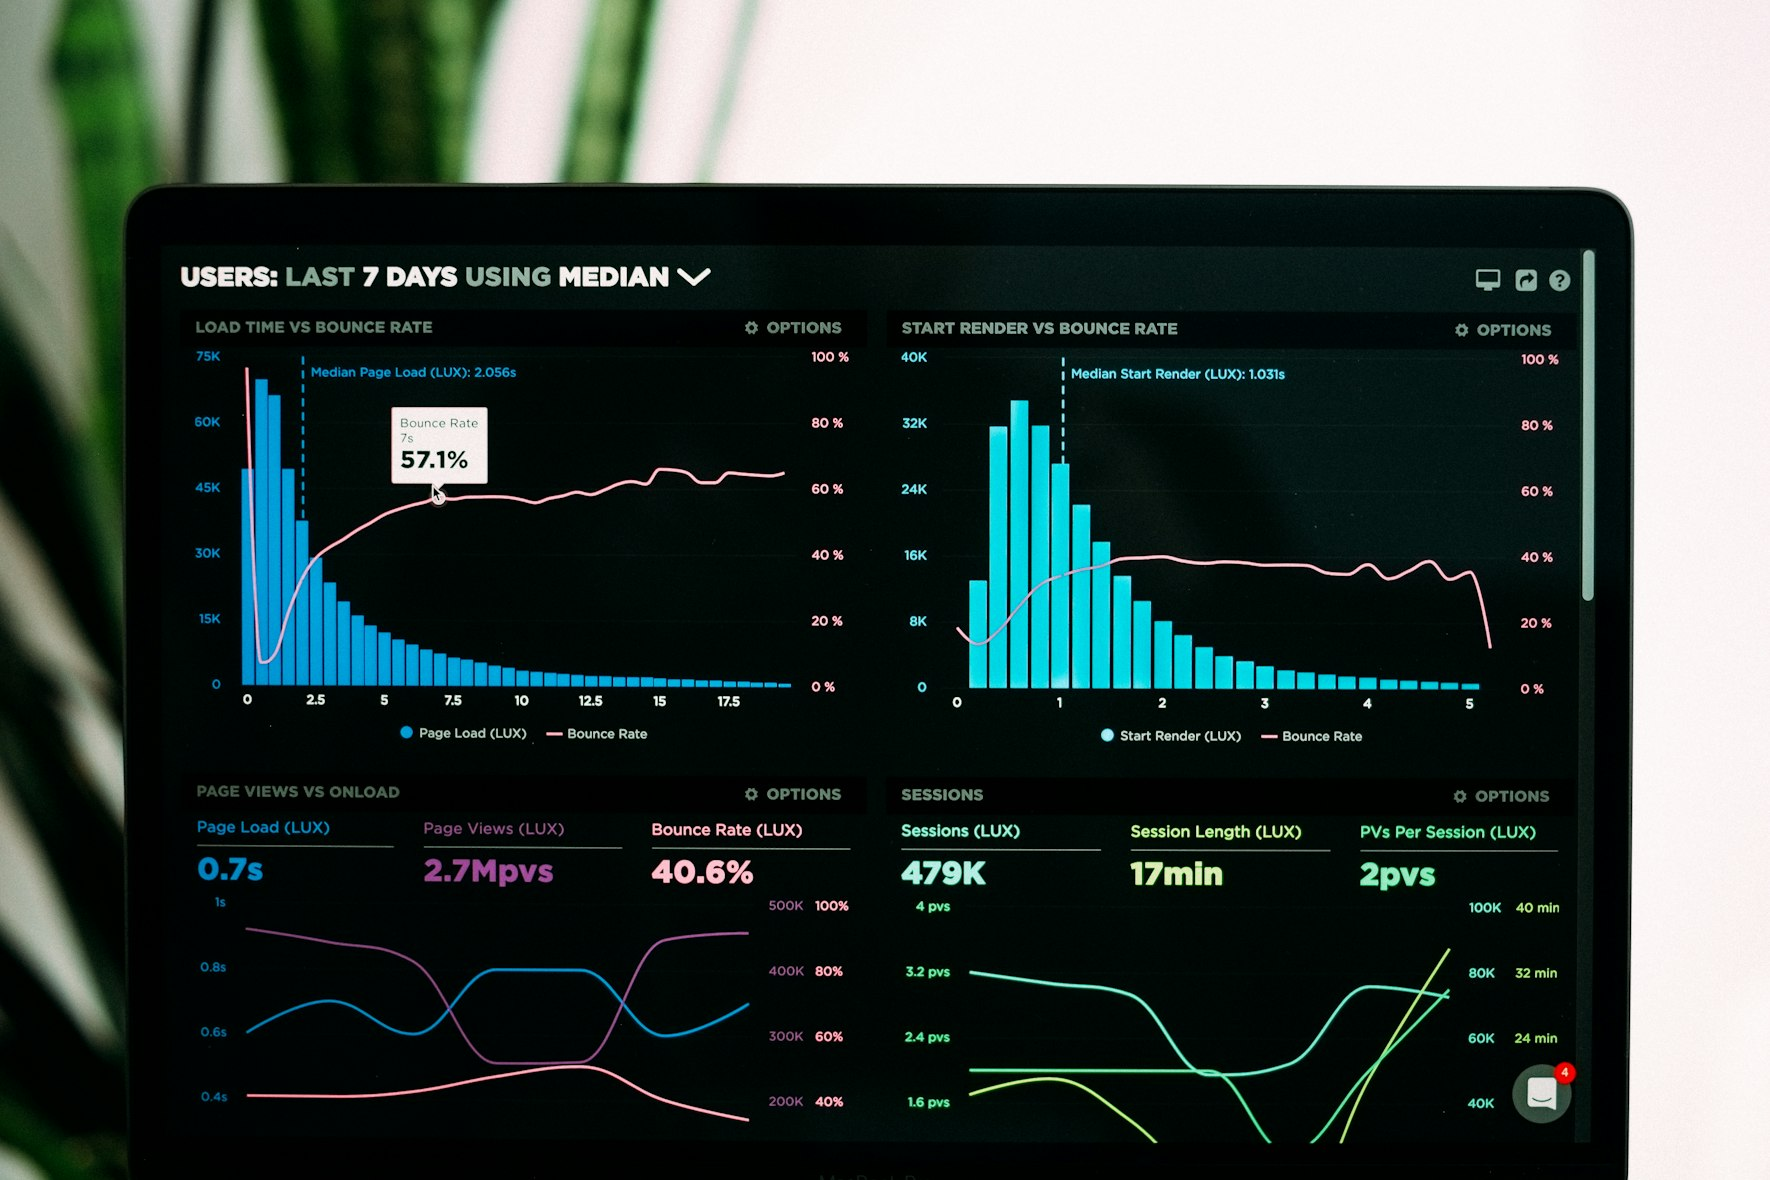
\includegraphics{index_files/mediabag/photo-1551288049-beb.jpg}

\begin{center}\rule{0.5\linewidth}{0.5pt}\end{center}

\hypertarget{types-of-research-design}{%
\subsection{\texorpdfstring{{6} {Types of Research
Design}}{6 Types of Research Design}}\label{types-of-research-design}}

\textbf{Key concepts to distinguish studies:}

\begin{itemize}
\tightlist
\item
  \textbf{Purpose}: Descriptive vs.~analytical
\item
  \textbf{Investigator control}: Observational vs.~interventional
\item
  \textbf{Directionality}: Forward vs.~backward
\item
  \textbf{Sample selection}: Based on exposure, disease, or neither
\item
  \textbf{Timing}: Prospective vs.~retrospective
\end{itemize}

\textbf{Study Types:} - Cross-sectional - Case-control - Retrospective
cohort - Prospective cohort - Randomized controlled trial (RCT)

\begin{center}\rule{0.5\linewidth}{0.5pt}\end{center}

\hypertarget{basic-terminology-exposure-and-disease}{%
\subsection{\texorpdfstring{{7} {Basic Terminology: Exposure and
Disease}}{7 Basic Terminology: Exposure and Disease}}\label{basic-terminology-exposure-and-disease}}

\begin{itemize}
\tightlist
\item
  \textbf{E} = ``Exposure''

  \begin{itemize}
  \tightlist
  \item
    Risk factor (e.g., smoking, occupational hazard)
  \item
    Intervention (e.g., drug, prevention program)
  \end{itemize}
\item
  \textbf{D} = ``Disease'' or outcome

  \begin{itemize}
  \tightlist
  \item
    Disease, injury, death
  \item
    Any health-related outcome
  \end{itemize}
\item
  \textbf{E₀} and \textbf{D₀} = Absence of exposure/disease
\item
  \textbf{E₁} and \textbf{D₁} = Presence of exposure/disease
\end{itemize}

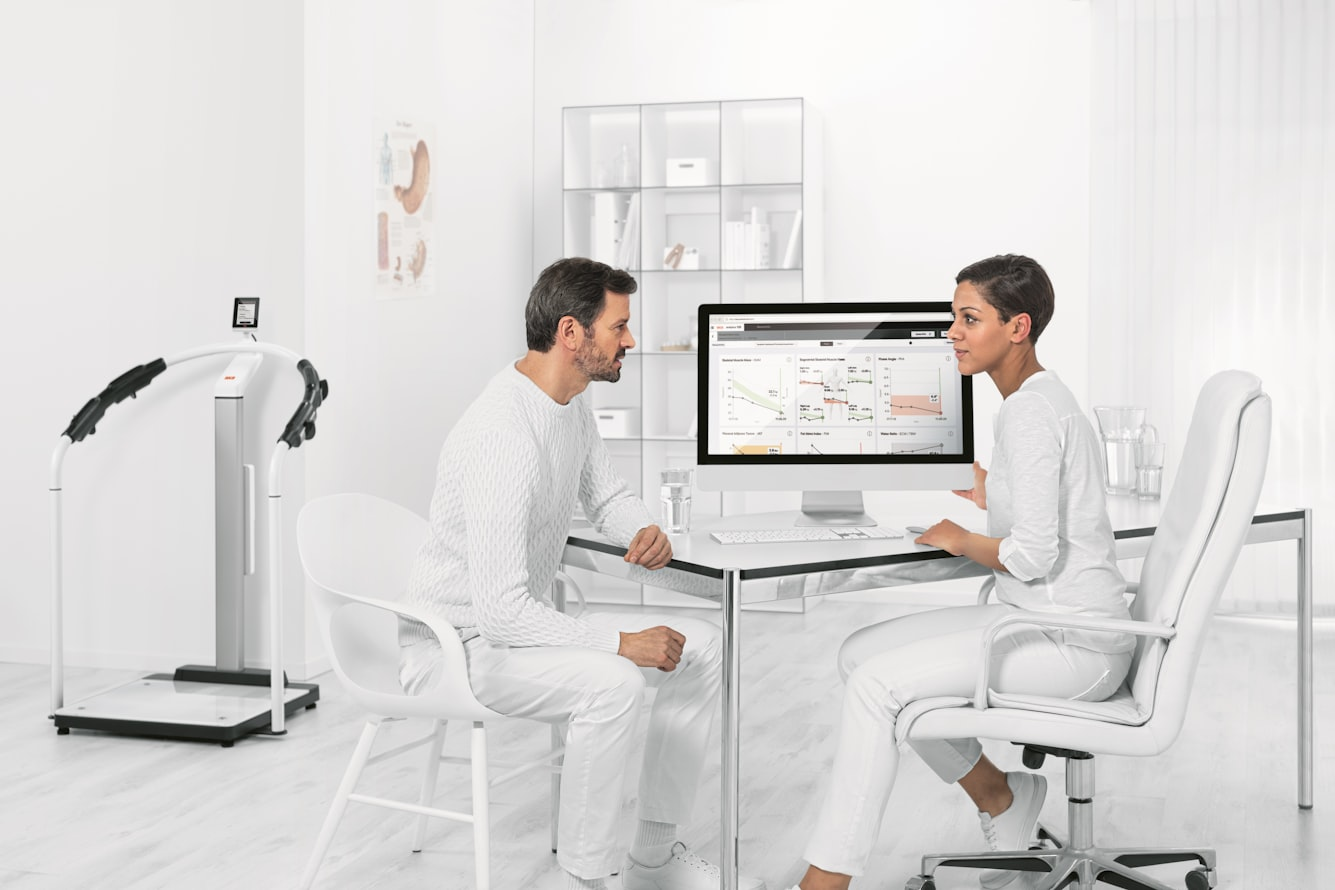
\includegraphics{index_files/mediabag/photo-1589279003513-.jpg}

This basic E and D framework helps illustrate the logic behind different
epidemiological study designs.

\begin{center}\rule{0.5\linewidth}{0.5pt}\end{center}

\hypertarget{study-designs-summary}{%
\subsection{\texorpdfstring{{8} {Study Designs
Summary}}{8 Study Designs Summary}}\label{study-designs-summary}}

\begin{longtable}[]{@{}
  >{\raggedright\arraybackslash}p{(\columnwidth - 10\tabcolsep) * \real{0.2137}}
  >{\raggedright\arraybackslash}p{(\columnwidth - 10\tabcolsep) * \real{0.1880}}
  >{\raggedright\arraybackslash}p{(\columnwidth - 10\tabcolsep) * \real{0.1538}}
  >{\raggedright\arraybackslash}p{(\columnwidth - 10\tabcolsep) * \real{0.1368}}
  >{\raggedright\arraybackslash}p{(\columnwidth - 10\tabcolsep) * \real{0.1880}}
  >{\raggedright\arraybackslash}p{(\columnwidth - 10\tabcolsep) * \real{0.1197}}@{}}
\toprule\noalign{}
\begin{minipage}[b]{\linewidth}\raggedright
Study Type
\end{minipage} & \begin{minipage}[b]{\linewidth}\raggedright
Purpose
\end{minipage} & \begin{minipage}[b]{\linewidth}\raggedright
Control
\end{minipage} & \begin{minipage}[b]{\linewidth}\raggedright
Directionality
\end{minipage} & \begin{minipage}[b]{\linewidth}\raggedright
Sample Selection
\end{minipage} & \begin{minipage}[b]{\linewidth}\raggedright
Timing
\end{minipage} \\
\midrule\noalign{}
\endhead
\bottomrule\noalign{}
\endlastfoot
\textbf{Cross-sectional} & Descriptive/Analytical & Observational &
Concurrent & Representative sample & Retrospective \\
\textbf{Case-control} & Analytical & Observational & Backward & Based on
disease & Retrospective \\
\textbf{Retrospective cohort} & Analytical & Observational & Forward &
Based on exposure & Retrospective \\
\textbf{Prospective cohort} & Analytical & Observational & Forward &
Based on exposure & Prospective \\
\textbf{Randomized control trial} & Analytical & Interventional &
Forward & Based on exposure & Prospective \\
\end{longtable}

\begin{center}\rule{0.5\linewidth}{0.5pt}\end{center}

\hypertarget{cross-sectional-studies}{%
\subsection{\texorpdfstring{{9} {Cross-Sectional
Studies}}{9 Cross-Sectional Studies}}\label{cross-sectional-studies}}

\begin{itemize}
\tightlist
\item
  Also called \textbf{prevalence studies}
\item
  Exposure and outcome assessed \textbf{simultaneously}
\item
  Can be descriptive or analytical
\item
  Provides a ``snapshot'' of a population
\item
  Relatively quick and inexpensive
\end{itemize}

\textbf{Limitations}:

\begin{itemize}
\item
  Cannot establish temporal sequence
\item
  Only includes survivors of disease
\item
  Not suitable for rare diseases
\end{itemize}

\includegraphics{imgs/crossSection.jpg}

\emph{A snapshot in time: both exposure and outcome measured
simultaneously}

\begin{center}\rule{0.5\linewidth}{0.5pt}\end{center}

\hypertarget{in-class-exercise}{%
\subsection{\texorpdfstring{{10} {In-class
exercise}}{10 In-class exercise}}\label{in-class-exercise}}

\begin{center}\rule{0.5\linewidth}{0.5pt}\end{center}

\hypertarget{case-control-analysis}{%
\subsection{\texorpdfstring{{11} {Case-Control
Analysis}}{11 Case-Control Analysis}}\label{case-control-analysis}}

\begin{itemize}
\tightlist
\item
  Cannot directly compute relative risk
\item
  Use \textbf{odds ratio (OR)} as an estimate:
\end{itemize}

\[OR = \frac{ad}{bc}\]

\begin{itemize}
\tightlist
\item
  In a 2×2 table:
\end{itemize}

\[
\begin{array}{|c|c|c|} \hline
 & D_1 & D_0 \\ \hline
E_1 & a & b \\ \hline
E_0 & c & d \\ \hline
\end{array}
\]

\begin{itemize}
\tightlist
\item
  When disease is rare, OR ≈ RR
\end{itemize}

\includegraphics{imgs/caseControl.png}

What is happening here?

\begin{center}\rule{0.5\linewidth}{0.5pt}\end{center}

\hypertarget{cohort-studies}{%
\subsection{\texorpdfstring{{12} {Cohort
Studies}}{12 Cohort Studies}}\label{cohort-studies}}

\begin{itemize}
\tightlist
\item
  Start with \textbf{exposure status} (E₁ and E₀)
\item
  Follow forward to observe outcome
\item
  Two types:

  \begin{itemize}
  \tightlist
  \item
    \textbf{Prospective}: Start now, follow into future
  \item
    \textbf{Retrospective}: Look back at historical exposure
  \end{itemize}
\item
  Can study multiple outcomes
\item
  Directly computes incidence and relative risk
\end{itemize}

\includegraphics{imgs/cohort.jpg}

\emph{Following groups forward from exposure to outcome}

\begin{center}\rule{0.5\linewidth}{0.5pt}\end{center}

\hypertarget{cohort-analysis}{%
\subsection{\texorpdfstring{{13} {Cohort
Analysis}}{13 Cohort Analysis}}\label{cohort-analysis}}

\begin{itemize}
\tightlist
\item
  \textbf{Relative Risk (RR)} quantifies association between exposure
  and outcome:
\end{itemize}

\[RR = \frac{a/(a+b)}{c/(c+d)}\]

\begin{itemize}
\tightlist
\item
  In a 2×2 table:
\end{itemize}

\[
\begin{array}{|c|c|c|} \hline
 & D_1 & D_0 \\ \hline
E_1 & a & b \\ \hline
E_0 & c & d \\ \hline
\end{array}
\]

\begin{itemize}
\tightlist
\item
  Allows for:

  \begin{itemize}
  \tightlist
  \item
    Direct incidence calculation
  \item
    Assessment of multiple outcomes
  \item
    Use with rare exposures
  \end{itemize}
\end{itemize}

\textbf{Challenges:}

\begin{itemize}
\item
  Time-consuming and costly
\item
  Potential for loss to follow-up
\item
  Not ideal for rare diseases
\item
  Diagnostic changes over time may affect results
\end{itemize}

\begin{center}\rule{0.5\linewidth}{0.5pt}\end{center}

\hypertarget{randomized-controlled-trials-rcts}{%
\subsection{\texorpdfstring{{14} {Randomized Controlled Trials
(RCTs)}}{14 Randomized Controlled Trials (RCTs)}}\label{randomized-controlled-trials-rcts}}

\begin{itemize}
\tightlist
\item
  \textbf{Gold standard} for assessing causal relationships
\item
  Participants randomly allocated to intervention (E₁) or control (E₀)
\item
  Minimizes confounding and bias through:

  \begin{itemize}
  \tightlist
  \item
    Randomization
  \item
    Blinding (single, double)
  \end{itemize}
\item
  Can be conducted at individual or group level
\end{itemize}

\textbf{Phases of clinical trials:}

\begin{itemize}
\item
  \textbf{Phase I:} Safety and dosage (small sample)
\item
  \textbf{Phase II:} Effectiveness and side effects
\item
  \textbf{Phase III:} Confirm effectiveness, monitor adverse reactions
  (RCT)
\item
  \textbf{Phase IV:} Post-marketing surveillance
\end{itemize}

\emph{Randomization helps balance known and unknown confounders.}

\begin{center}\rule{0.5\linewidth}{0.5pt}\end{center}

\hypertarget{validity-and-reliability}{%
\subsection{\texorpdfstring{{15} {Validity and
Reliability}}{15 Validity and Reliability}}\label{validity-and-reliability}}

\textbf{Measurement Validity}

\begin{itemize}
\item
  \textbf{Face validity}: Appears reasonable on the surface
\item
  \textbf{Content validity}: Covers full scope of concept
\item
  \textbf{Construct validity}: Reflects theoretical concept
\item
  \textbf{Criterion validity}: Correlates with external standard
\item
  \textbf{Concurrent validity}: Correlates with present condition
\item
  \textbf{Predictive validity}: Forecasts future outcome
\end{itemize}

\textbf{Study Validity}

\begin{itemize}
\item
  \textbf{Internal validity}: Results valid for study sample
\item
  \textbf{External validity}: Results generalize to other populations
\end{itemize}

\textbf{Reliability}

\begin{itemize}
\item
  \textbf{Test-retest}: Same test, different times
\item
  \textbf{Inter-observer}: Different observers agree
\item
  \textbf{Intra-observer}: Same observer consistent over time
\end{itemize}

\begin{center}\rule{0.5\linewidth}{0.5pt}\end{center}

\hypertarget{reliability-vs.-validity}{%
\subsection{\texorpdfstring{{16} {Reliability
vs.~Validity}}{16 Reliability vs.~Validity}}\label{reliability-vs.-validity}}

\begin{itemize}
\tightlist
\item
  \textbf{Reliability} = consistency of measurement
\item
  \textbf{Validity} = accuracy of what is intended to be measured
\item
  A tool can be reliable but not valid
\item
  A tool cannot be valid if it is not reliable
\end{itemize}

\begin{figure}

{\centering \includegraphics{index_files/mediabag/1024px-Reliability_a.png}

}

\caption{Target analogy for validity and reliability}

\end{figure}

\begin{center}\rule{0.5\linewidth}{0.5pt}\end{center}

\hypertarget{types-of-error}{%
\subsection{\texorpdfstring{{17} {Types of
Error}}{17 Types of Error}}\label{types-of-error}}

\textbf{Random Error}

\begin{itemize}
\item
  Caused by chance or sampling variation
\item
  Affects \textbf{precision}
\item
  Can be reduced by increasing sample size
\item
  Produces unpredictable fluctuations
\end{itemize}

\textbf{Systematic Error (Bias)}

\begin{itemize}
\item
  Consistent, repeatable error due to flaws in design or measurement
\item
  Affects \textbf{validity}
\item
  Not reduced by increasing sample size
\item
  Must be addressed in study design
\end{itemize}

\begin{center}\rule{0.5\linewidth}{0.5pt}\end{center}

\hypertarget{major-types-of-bias}{%
\subsection{\texorpdfstring{{18} {Major Types of
Bias}}{18 Major Types of Bias}}\label{major-types-of-bias}}

\subsubsection{Selection Bias}

\begin{itemize}
\tightlist
\item
  Systematic differences between those selected and not selected
\item
  Examples:

  \begin{itemize}
  \tightlist
  \item
    Low response rate
  \end{itemize}
\item
  Healthy worker effect
\item
  Volunteer bias
\item
  Berkson's bias (hospital sampling)

  \begin{itemize}
  \tightlist
  \item
    Loss to follow-up
  \item
    Survivor bias
  \end{itemize}
\end{itemize}

\subsubsection{Information Bias}

\begin{itemize}
\tightlist
\item
  Measurement error or misclassification
\item
  Examples:

  \begin{itemize}
  \tightlist
  \item
    Recall bias
  \item
    Observer/interviewer bias
  \item
    Social desirability bias
  \item
    Instrument bias
  \item
    Diagnostic suspicion bias
  \end{itemize}
\end{itemize}

\subsubsection{Confounding}

\begin{itemize}
\tightlist
\item
  Third variable distorts exposure-outcome relationship
\item
  Must be:

  \begin{enumerate}
  \def\labelenumi{\arabic{enumi}.}
  \tightlist
  \item
    Associated with exposure
  \item
    Risk factor for the outcome
  \item
    Not an intermediate step in the causal path
  \end{enumerate}
\end{itemize}

\begin{center}\rule{0.5\linewidth}{0.5pt}\end{center}

\hypertarget{controlling-for-confounding}{%
\subsection{\texorpdfstring{{19} {Controlling for
Confounding}}{19 Controlling for Confounding}}\label{controlling-for-confounding}}

\textbf{At Design Stage}

\begin{enumerate}
\def\labelenumi{\arabic{enumi}.}
\tightlist
\item
  \textbf{Randomization}

  \begin{itemize}
  \tightlist
  \item
    Evenly distributes confounders across groups
  \end{itemize}
\item
  \textbf{Restriction}

  \begin{itemize}
  \tightlist
  \item
    Limit study to specific subgroup
  \end{itemize}
\item
  \textbf{Matching}

  \begin{itemize}
  \tightlist
  \item
    Pair participants with similar characteristics
  \end{itemize}
\end{enumerate}

\textbf{At Analysis Stage}

\begin{enumerate}
\def\labelenumi{\arabic{enumi}.}
\setcounter{enumi}{3}
\tightlist
\item
  \textbf{Stratification}

  \begin{itemize}
  \tightlist
  \item
    Analyze within homogeneous strata\\
  \item
    Mantel-Haenszel summary estimate
  \end{itemize}
\item
  \textbf{Multivariable Modeling}

  \begin{itemize}
  \tightlist
  \item
    Include confounders as covariates\\
  \item
    Logistic regression, Cox models
  \end{itemize}
\end{enumerate}

\begin{center}\rule{0.5\linewidth}{0.5pt}\end{center}

\hypertarget{effect-modification-interaction}{%
\subsection{\texorpdfstring{{20} {Effect Modification
(Interaction)}}{20 Effect Modification (Interaction)}}\label{effect-modification-interaction}}

\begin{itemize}
\tightlist
\item
  Occurs when the effect of exposure differs across levels of a third
  variable
\item
  \textbf{Not the same as confounding}
\item
  Can be additive or multiplicative
\item
  \textbf{Additive Model:}\\
  \[RREM = RRE + RRM - 1\]
\item
  \textbf{Multiplicative Model:}\\
  \[RREM = RRE \times RRM\]
\item
  Interpretation:

  \begin{itemize}
  \tightlist
  \item
    If RREM \textgreater{} expected → \textbf{synergism}
  \item
    If RREM \textless{} expected → \textbf{antagonism}
  \end{itemize}
\end{itemize}

\textbf{Example:} Asbestos and smoking on lung cancer risk
\includegraphics{imgs/effectModification.png}

\begin{center}\rule{0.5\linewidth}{0.5pt}\end{center}

\hypertarget{qualitative-methods}{%
\subsection{\texorpdfstring{{21} {Qualitative
Methods}}{21 Qualitative Methods}}\label{qualitative-methods}}

\begin{itemize}
\tightlist
\item
  Originates from the social sciences
\item
  Explores perceptions, beliefs, experiences
\item
  Often used to:

  \begin{itemize}
  \tightlist
  \item
    Understand lived experiences
  \item
    Explore context and meaning
  \item
    Inform survey and tool development
  \end{itemize}
\item
  \textbf{Common techniques:}

  \begin{itemize}
  \tightlist
  \item
    In-depth interviews
  \item
    Focus groups
  \item
    Participant observation
  \item
    Document analysis
  \end{itemize}
\end{itemize}

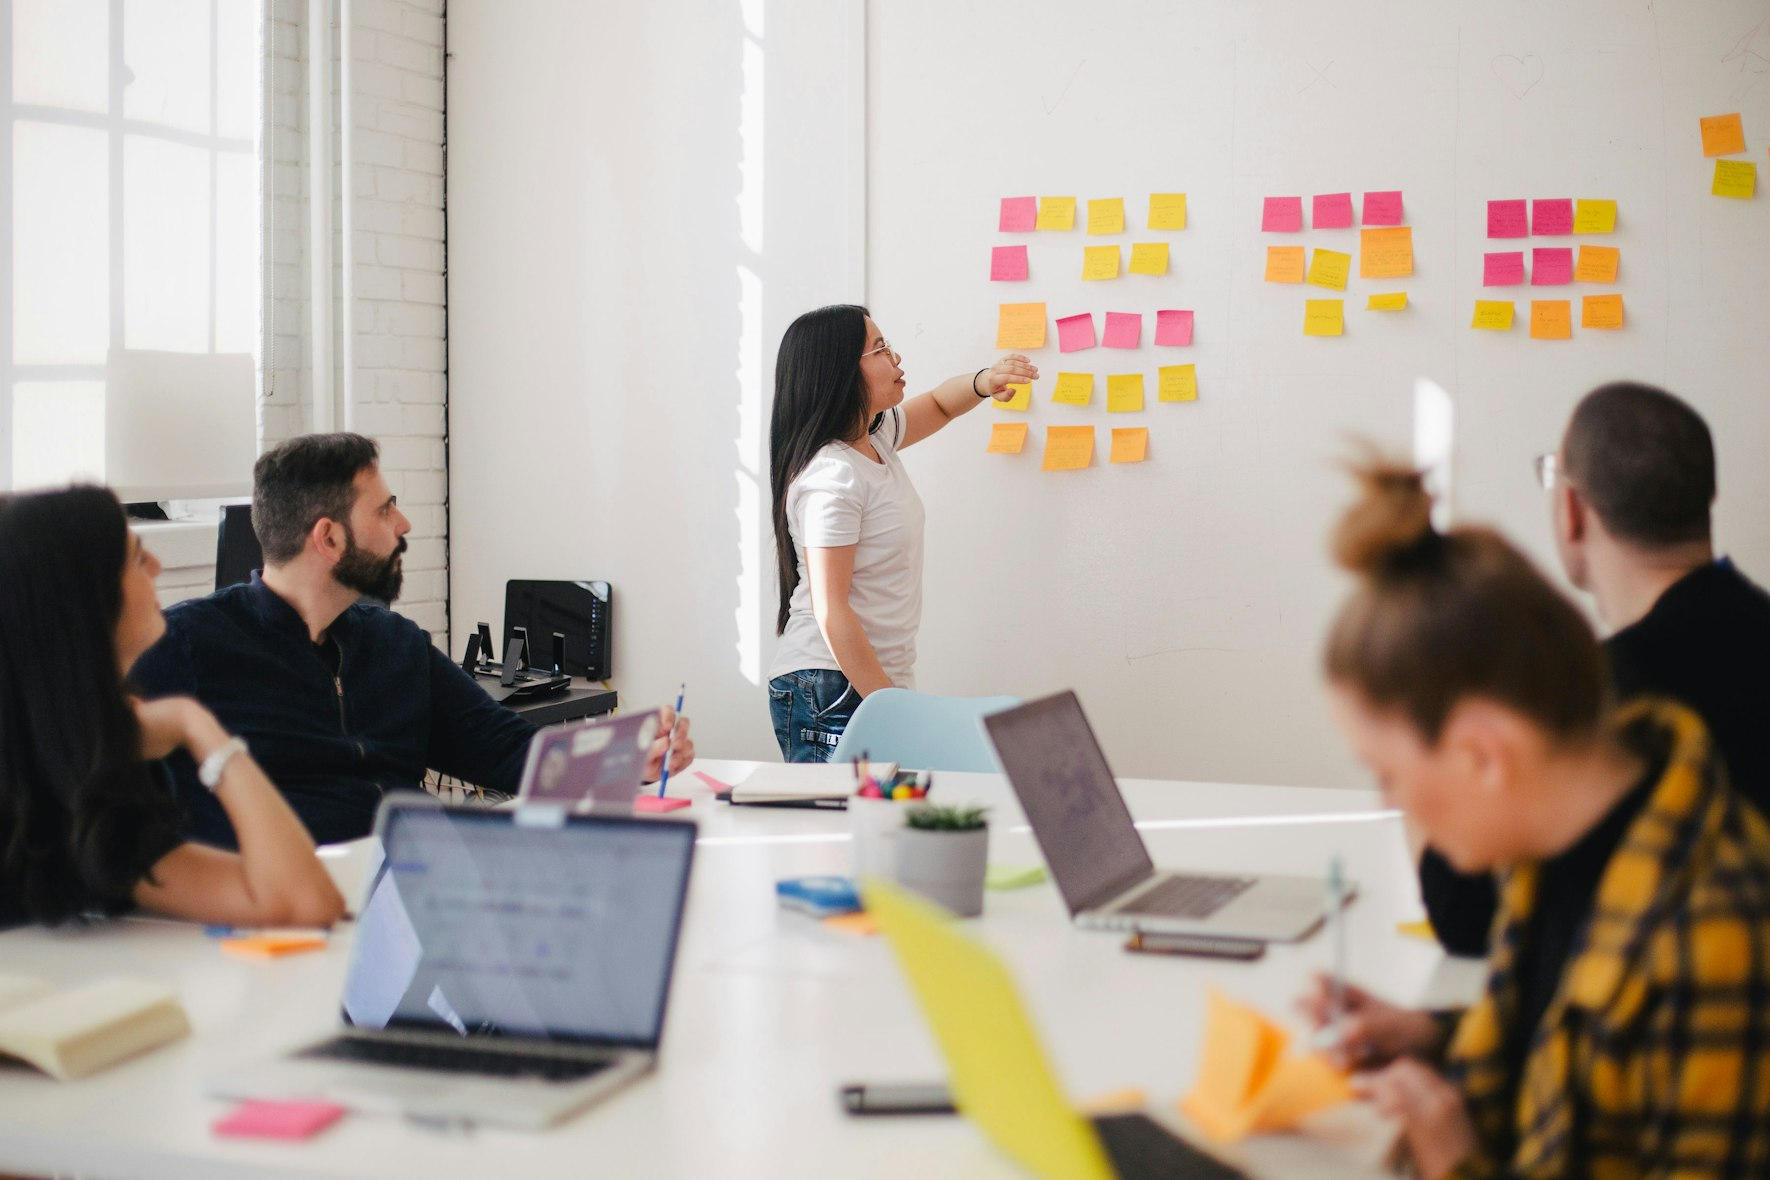
\includegraphics{index_files/mediabag/photo-1552664730-d30.jpg}

\emph{Mixed methods combine qualitative insight with quantitative data.}

\begin{center}\rule{0.5\linewidth}{0.5pt}\end{center}

\hypertarget{types-of-qualitative-methods}{%
\subsection{\texorpdfstring{{22} {Types of Qualitative
Methods}}{22 Types of Qualitative Methods}}\label{types-of-qualitative-methods}}

\subsubsection{Observation}

\begin{itemize}
\tightlist
\item
  \textbf{Participant observation}: Researcher immersed in environment
\item
  Captures real behavior and interactions
\item
  Varies in degree of participation
\end{itemize}

\subsubsection{Interviews}

\begin{itemize}
\tightlist
\item
  \textbf{Structured}: Same questions for all
\item
  \textbf{Semi-structured}: Flexible, guided
\item
  \textbf{In-depth}: Deep exploration
\item
  \textbf{Focus groups}: Group discussion dynamics
\end{itemize}

\subsubsection{Document Analysis}

\begin{itemize}
\tightlist
\item
  Systematic review of written or visual materials
\item
  Examples:

  \begin{itemize}
  \tightlist
  \item
    Public records, policy reports
  \item
    Personal journals, media, videos
  \end{itemize}
\end{itemize}

\begin{center}\rule{0.5\linewidth}{0.5pt}\end{center}

\hypertarget{integrating-qualitative-quantitative-methods}{%
\subsection{\texorpdfstring{{23} {Integrating Qualitative \&
Quantitative
Methods}}{23 Integrating Qualitative \& Quantitative Methods}}\label{integrating-qualitative-quantitative-methods}}

\textbf{Ways to integrate qualitative methods:}

\begin{enumerate}
\def\labelenumi{\arabic{enumi}.}
\item
  \textbf{Pre-study}: To develop hypotheses or instruments
\item
  \textbf{During study}: To explain unexpected results
\item
  \textbf{Post-study}: To interpret and validate findings
\item
  \textbf{Standalone}: As an alternative or complement to quantitative
\end{enumerate}

\textbf{Example: Regional Health Needs Assessment}

\begin{itemize}
\item
  \textbf{Quantitative}: Epidemiologic data, service access
\item
  \textbf{Qualitative}: Focus groups with residents, interviews with key
  informants
\end{itemize}


\includegraphics{index_files/mediabag/photo-1544027993-37d.jpg}

\emph{Combining methods gives depth and context.}

\begin{center}\rule{0.5\linewidth}{0.5pt}\end{center}

\hypertarget{ethical-considerations}{%
\subsection{\texorpdfstring{{24} {Ethical
Considerations}}{24 Ethical Considerations}}\label{ethical-considerations}}

\textbf{Four Ethical Principles:}

\begin{enumerate}
\def\labelenumi{\arabic{enumi}.}
\item
  \textbf{Autonomy} -- Respect for individuals
\item
  \textbf{Beneficence} -- Maximize benefits
\item
  \textbf{Non-maleficence} -- Do no harm
\item
  \textbf{Justice} -- Fair treatment and burden distribution
\end{enumerate}

\textbf{Research Protections:}

\begin{itemize}
\item
  Informed consent
\item
  Confidentiality
\item
  Data security
\item
  Vulnerable populations
\item
  Institutional Review Boards (IRBs)
\item
  Research integrity and transparency
\end{itemize}

\begin{center}\rule{0.5\linewidth}{0.5pt}\end{center}

\hypertarget{key-takeaways}{%
\subsection{\texorpdfstring{{25} {Key
Takeaways}}{25 Key Takeaways}}\label{key-takeaways}}

\begin{itemize}
\tightlist
\item
  Choose the study design that best answers your research question
\item
  Recognize and control for bias and confounding
\item
  Understand the role of validity and reliability
\item
  Combine methods when appropriate
\item
  Always prioritize ethics and participant rights
\end{itemize}


\includegraphics{index_files/mediabag/photo-1517245386807-.jpg}

\begin{quote}
``No method is inherently superior---it all depends on the research
question.'' -- T. Kue Young
\end{quote}



\end{document}
